The HL-LHC upgrade will require major changes to ATLAS Tile Calorimeter electronics and data readout.  UTA will construct half of the Tile Calorimeter pre-processor boards, which provide an important interface between on-detector electronics and the data acquisition and trigger systems. Currently, the other half of the boards will be provided by the University of Valencia. The two institutions are collaborating on the design and R\&D. This project is an important responsibility in the HL-LHC Upgrade project, and under the coordination of US ATLAS management.

For this project, we will perform the design and fabrication of the Trigger DAQ interface (TDAQi) blades which are the rear transition modules of the Tile calorimeter back-end preprocessor (PPR). These boards configure the processed data from the front-end electronics and route data to the DAQ system via the FELIX module and to the L0/L1 Calo and Muon trigger system through dedicated links. UTA is responsible for the production of 32 boards. Additional tasks are parts procurement, monitoring of outsourced assembly, burn-in of cards in a dedicated setup with validation testing and repairs when needed, and installation and commissioning at CERN. This activitiy is funded through the US ATLAS HL-LHC construction and upgrade R\&D projects. PI De and postdoctoral researcher Usai, both of whom partially funded through the base program, will be managing this project.
In Figure~\ref{ppr_proto} we show the current prototype of the PPR TDAQi board.

\begin{figure}[hbt]
\begin{center}
  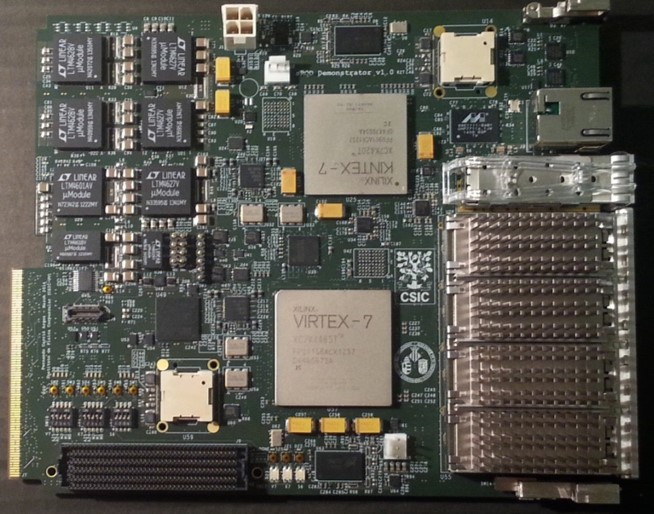
\includegraphics[width=4in]{De/atl_ppr_proto.jpg}
  \caption{Prototype of the TileCal PPR TDAQi board being deigned for HL-LHC at UTA in collaboration with the University of Valencia.}
  \label{ppr_proto}
\end{center}
\end{figure}

During the period of this base proposal, 2017-20, we will focus on design and prototyping work, setting up test stands, validating the prototypes, finalizing the design, and begin pre-production activities. Fabrication of the boards will begin in 2021.